\documentclass[a4paper]{article}
\usepackage{preamble}
\usepackage[spanish]{babel}

\setlength{\parskip}{\baselineskip}
\setlength{\parindent}{0pt}

\begin{document}
\pagestyle{fancy}

\section{Cálculo Teórico}

Se da un BJT y dos fuentes de voltage.

Para el BJT:
$$
\beta_{\text{lineal}}=300,\hspace{4ex}V_{BE\text{ umbral}}=0.6V,\hspace{4ex}V_{CE\text{ sat}}=0.12V
$$

El voltage $V_{1}$ varía entre $[0:5]V$, el voltage $V_{2}=5V$, la resistencia $R_{B}=40000\,\Omega=40\,k\Omega$ y la resistencia $R_{C}=2000\Omega=2\,k\Omega$.

Se pide:
\begin{align*}
\hspace{4ex}\triangleright\hspace{1ex}V_{1}\text{ vs }V_{CE} 
\hspace{4ex}\triangleright\hspace{1ex}V_{1}\text{ vs }I_{B}
\hspace{4ex}\triangleright\hspace{1ex}V_{1}\text{ vs }I_{C}
\hspace{4ex}\triangleright\hspace{1ex}V_{1}\text{ vs }\beta
\end{align*}

Conociendo $V_{BE}=0.6V$ y según la \textit{Ley de Ohm}
\begin{align}
I_{B}(V_{1})&=\frac{V_{1}-V_{BE \text{ umbral}}}{R_{B}}=\frac{[0'6:5]-0'6}{40000} \\
I_{B\text{ mín}}(V_{1}=0V)&=- \frac{0'6-0'6}{40000}=0\,\mu A \\
I_{B\text{ máx}}(V_{1}=5V)&=\frac{4'4}{40000}=1.1\times 10^{-4}\,A = 110\,\mu A
\end{align}
$$
\boxed{I_{B}=[0:110]\,\mu A}
$$
\begin{figure}[H]
    \centering
    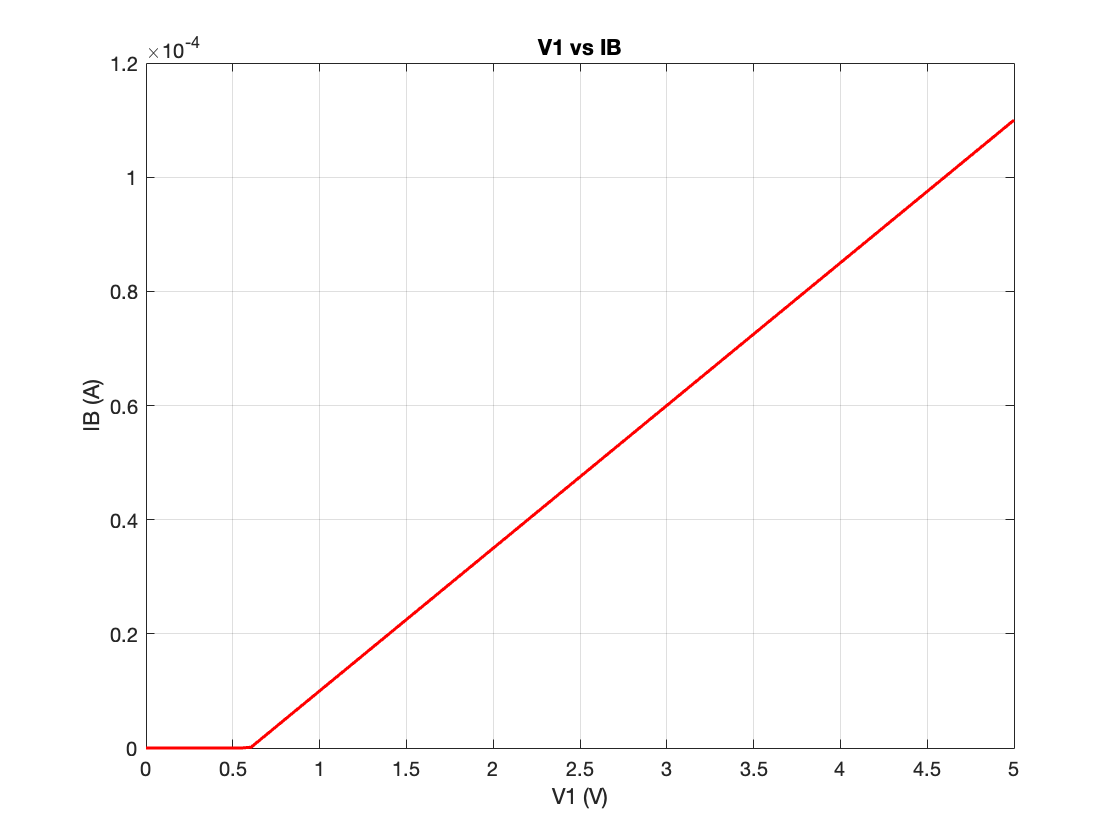
\includegraphics[width=0.9\textwidth]{IMG/bjt_2.png}
    \caption{$V_1\text{ vs }I_B$}
    \label{fig:bjt_2}
\end{figure}

\newpage

\begin{align}
I_{C}(I_{B})&=\beta \cdot I_{B} = 300\cdot [-15:100]\times 10^{-6} \\
I_{C\text{ mín}}(I_{B}=0\,\mu A) & =300\cdot 0=0\,mA \\
I_{C\text{ máx}}(I_{B}=110\,\mu A) & = 300\cdot 110\times 10^{-6}=0'03 = 33\,mA \\
\text{Saturation}\rightarrow V_{CE} &= V_2-I_C\cdot R_C =-61V \gg V_{CE\text{ sat}} \\
I_{C\text{saturado}} &= \frac{V_2-V_{CE\text{ sat}}}{R_C}=\frac{5-0'12}{2000}=2'44\,mA
\end{align}
$$
\boxed{I_{C}=[0:2.44]\,mA}
$$
\begin{figure}[H]
    \centering
    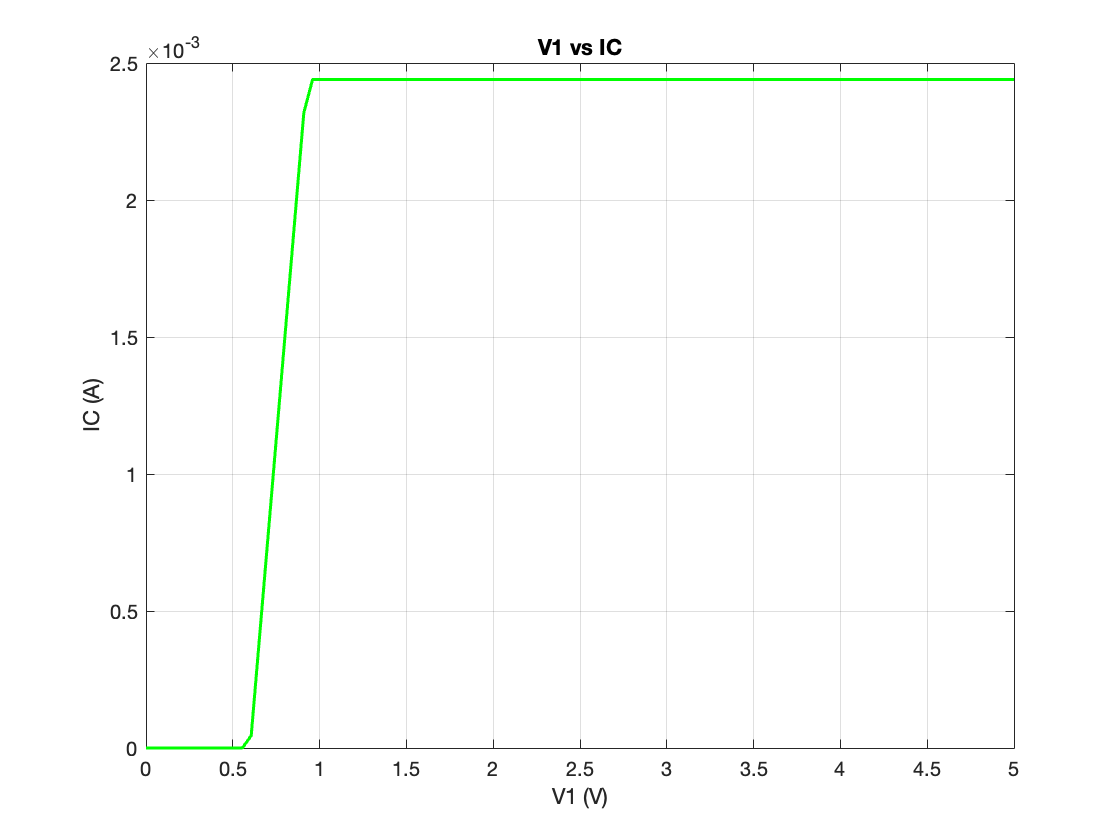
\includegraphics[width=0.9\textwidth]{IMG/bjt_3.png}
    \caption{$V_1\text{ vs }I_C$}
    \label{fig:bjt_3}
\end{figure}

\newpage

\begin{align}
V_{CE} & =V_{2}-I_{C}\cdot R_{C}=5-[0:33]\times 10^{-3}\cdot 2000 \\ 
V_{CE\text{ mín}}(I_{C}=33\,mA ) & =5-33\times 10^{-3}\cdot 2000=-61V \\
V_{CE\text{ máx}}(I_{C}=0\,mA) & =5-0\cdot 2000=5V
\end{align}
$$
\boxed{V_{CE}=[0.12:5]}
$$
ya que $V_{CE\text{ mín}}<V_{CE\text{ sat}}$.
\begin{figure}[H]
    \centering
    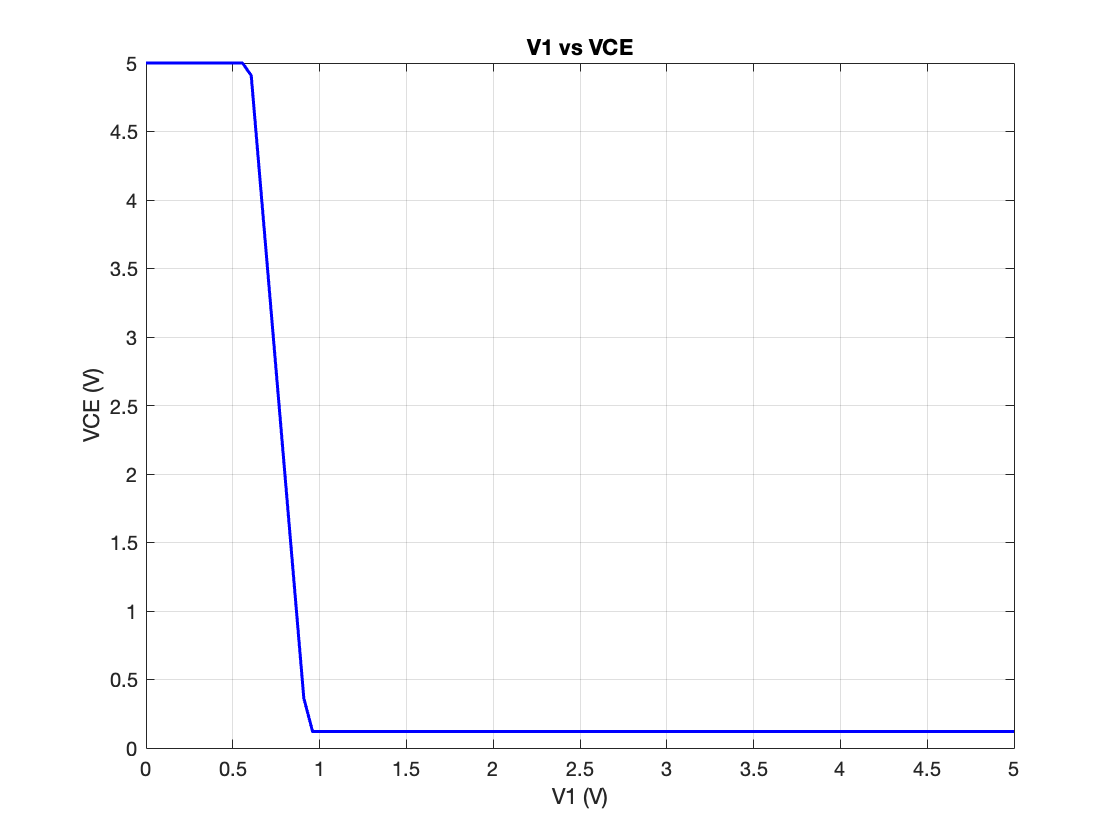
\includegraphics[width=0.9\textwidth]{IMG/bjt_1.png}
    \caption{$V_1\text{ vs }V_{CE}$}
    \label{fig:bjt_1}
\end{figure}

\newpage

\begin{align}
    \beta(I_C,I_B) &= \frac{I_C}{I_B} \\
    \beta_{\text{mín}}  &= 0 \\
    \beta_{\text{max}} &= \frac{330\times10^{-3}}{110\times10^{-6}}=300
\end{align}
$$
\boxed{\beta = [0:300]}
$$
\begin{figure}[H]
    \centering
    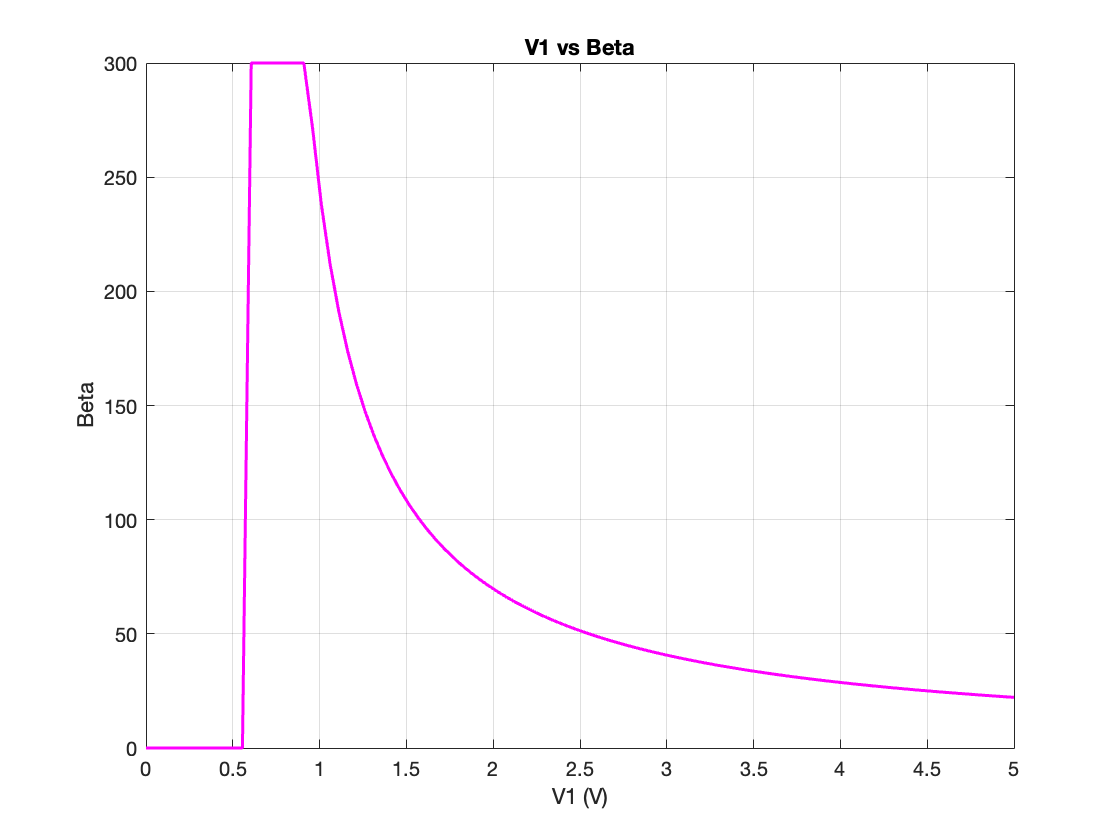
\includegraphics[width=0.9\textwidth]{IMG/bjt_4.png}
    \caption{$V_1\text{ vs }\mu$}
    \label{fig:bjt_4}
\end{figure}

Se produce una caída en $\beta$ cerca de $V_1=1V$ por la saturación en $I_C$.

\newpage

\section{Simulación LTspice}

\begin{minipage}{\textwidth}
    \begin{minipage}{0.49\textwidth}
        \begin{figure}[H]
            \centering
            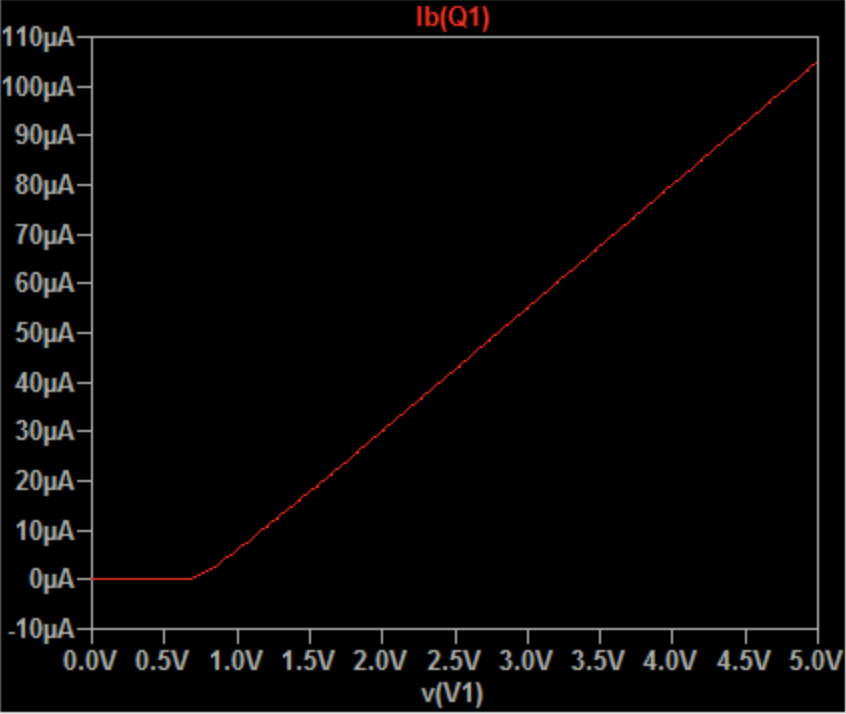
\includegraphics[width=\textwidth]{IMG/bjt_e_2.png}
            \caption{$V_1\text{ vs }I_B$ simulado}
            \label{fig:bjt_e_2}
        \end{figure}
    \end{minipage} \hfill
    \begin{minipage}{0.49\textwidth}
        \begin{figure}[H]
            \centering
            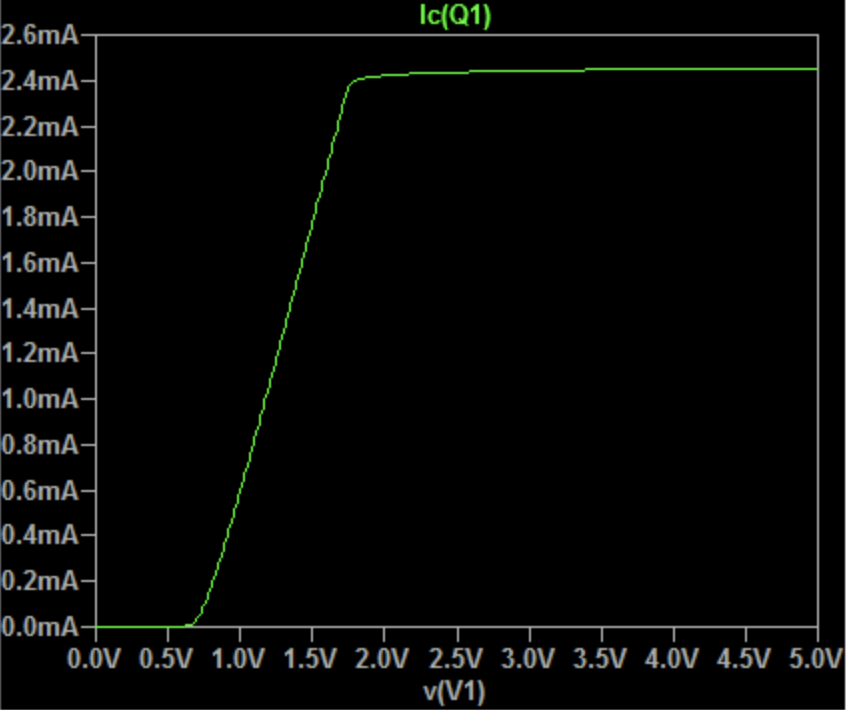
\includegraphics[width=\textwidth]{IMG/bjt_e_3.png}
            \caption{$V_1\text{ vs }I_C$ simulado}
            \label{fig:bjt_e_3}
        \end{figure}
    \end{minipage}
\end{minipage} \\
\begin{minipage}{\textwidth}
    \begin{minipage}{0.49\textwidth}
        \begin{figure}[H]
            \centering
            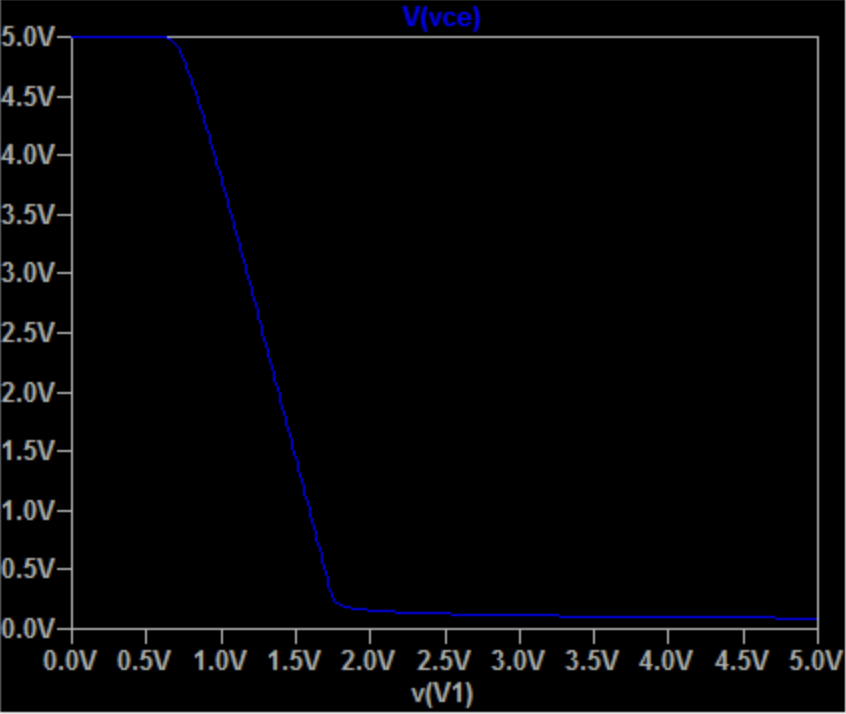
\includegraphics[width=\textwidth]{IMG/bjt_e_1.png}
            \caption{$V_1\text{ vs }V_{CE}$ simulado}
            \label{fig:bjt_e_1}
        \end{figure}
    \end{minipage}\hfill
    \begin{minipage}{0.49\textwidth}
        \begin{figure}[H]
            \centering
            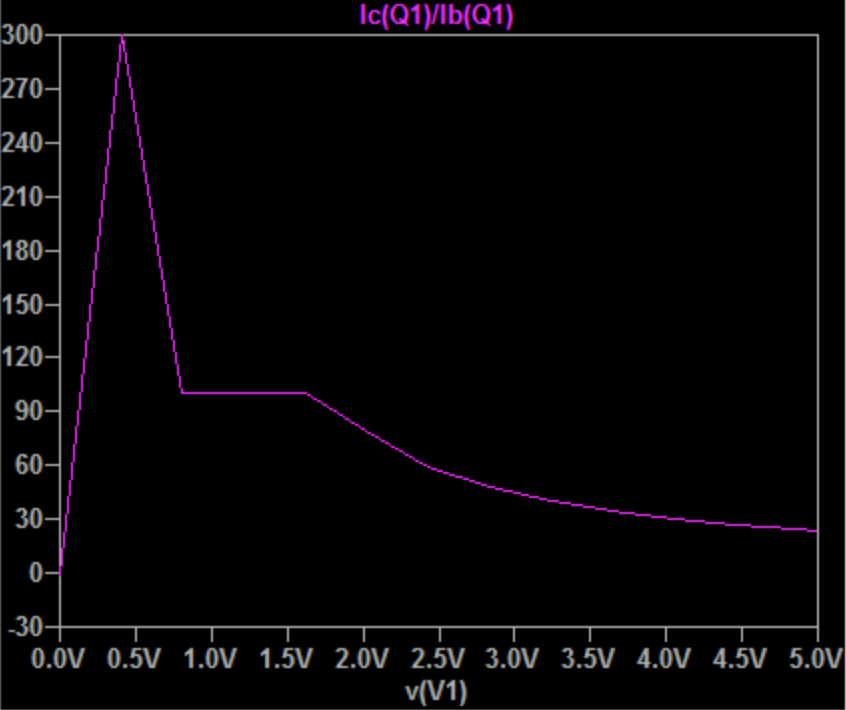
\includegraphics[width=\textwidth]{IMG/bjt_e_4.png}
            \caption{$V_1\text{ vs }\beta$ simulado}
            \label{fig:bjt_e_4}
        \end{figure}
    \end{minipage}
\end{minipage}

\end{document}
